\let\negmedspace\undefined
\let\negthickspace\undefined
\documentclass[journal]{IEEEtran}
\usepackage[a5paper, margin=10mm, onecolumn]{geometry}
\usepackage{tfrupee}
\setlength{\headheight}{1cm}
\setlength{\headsep}{0mm}
\usepackage{gvv-book}
\usepackage{gvv}
\usepackage{cite}
\usepackage{amsmath,amssymb,amsfonts,amsthm}
\usepackage{algorithmic}
\usepackage{graphicx}
\usepackage{float}
\usepackage{textcomp}
\usepackage{xcolor}
\usepackage{caption}
\usepackage{txfonts}
\usepackage{listings}
\usepackage{enumitem}
\usepackage{mathtools}
\usepackage{gensymb}
\usepackage{comment}
\usepackage[breaklinks=true]{hyperref}
\usepackage{tkz-euclide}
\usepackage{listings}
% \usepackage{gvv}
\def\inputGnumericTable{}
\usepackage[latin1]{inputenc}
\usepackage{color}
\usepackage{array}
\usepackage{longtable}
\usepackage{calc}
\usepackage{multirow}
\usepackage{hhline}
\usepackage{ifthen}
\usepackage{lscape}
\usepackage{tikz}
\usetikzlibrary{patterns}
\begin{document}
\bibliographystyle{IEEEtran}
\vspace{3cm}
\title{GATE 2012 MN }
\author{ai25btech11039
- Harichandana Varanasi}
\maketitle
% \maketitle
% \newpage
% \bigskip
{\let\newpage\relax\maketitle}
% \maketitle
% \newpage
% \bigskip
{\let\newpage\relax\maketitle}
\renewcommand{\thefigure}{\theenumi}
\renewcommand{\thetable}{\theenumi}
\setlength{\intextsep}{10pt} % Space between text and floats

\vspace{0.5em}
\begin{enumerate}[leftmargin=0pt]
\begin{center}
    {\Large \textbf{Duration: Three Hours \hfill Maximum Marks: 100}} \\
\end{center}
\noindent\textbf{\textit{Read the following instructions carefully.}}
   \item The computer allotted to you at the examination center runs a specialized software that permits only one answer to be selected for multiple choice questions using a mouse. Your answers shall be updated and saved on a server periodically and at the end of the examination.
    
    \item To login, enter your Registration Number and password provided in the envelope. Go through the symbols used in the test and understand the meaning before you start the examination. You can view all questions by clicking on the \textbf{View All Questions} button on the screen after the start of the examination.
    
    \item To answer a question, select the question using the selection panel on the screen and choose the correct answer by clicking on the radio button next to the answer. To change the answer, just click on another option. If you wish to leave a previously answered question unanswered, click on the button next to the selected option.
    
    \item The examination will automatically stop at the end of 3 hours.
    
    \item There are a total of 65 questions carrying 100 marks. Except questions Q.26–Q.30, all the other questions are of multiple choice type with only one correct answer. Questions Q.26–Q.30 require a numerical answer, and a number should be entered using the virtual keyboard on the monitor.
    
    \item Questions Q.1–Q.25 carry 1 mark each. Questions Q.26–Q.55 carry 2 marks each. The 2 marks questions include two pairs of common data questions and two pairs of linked answer questions. The answer to the second question of the linked answer questions depends on the answer to the first question of the pair. If the first question in the linked pair is wrongly answered or is unattempted, then the answer to the second question in the pair will not be evaluated.
    
    \item Questions Q.56–Q.65 belong to General Aptitude (GA) section and carry a total of 15 marks. Questions Q.56–Q.60 carry 1 mark each, and questions Q.61–Q.65 carry 2 marks each.
    
    \item Unattempted questions will result in zero mark and wrong answers will result in \textbf{NEGATIVE marks}. There is no negative marking for questions of numerical answer type, i.e., for Q.26–Q.30. For all 1 mark questions, $\tfrac{1}{3}$ mark will be deducted for each wrong answer. For all 2 marks questions, $\tfrac{2}{3}$ mark will be deducted for each wrong answer. However, in the case of the linked answer question pair, there will be negative marks only for wrong answer to the first question and no negative marks for the numerical answer to the second question.
    
    \item Calculator is disallowed. Charts, graph sheets or tables are \textbf{NOT} allowed in the examination hall. Do the rough work on the Scribble Pad provided.
    
    \item You must sign this sheet and leave it with the invigilators at the end of the examination.

\end{enumerate}

\noindent\textbf{Q.\,1 -- Q.\,25 carry one mark each.}\\[0.5em]
\begin{enumerate}[leftmargin=0pt]

% Q1
\item A 30 m steel tape having an area of cross-section of $5 \times 10^{-6}\,\text{m}^{2}$ is
standardized at $20\deg C$, supported under a tension of $5.45\,\text{N}$. It is used to measure a
horizontal distance of $81.15\,\text{m}$ under an applied tension of $9.09\,\text{N}$. The error,
due to incorrect pulling arrangement in this observation, in m is \\
$(E_{\text{steel}} = 200\,\text{GPa})$
\begin{multicols}{2}
\begin{enumerate}[label=(\Alph*), itemsep=0pt, topsep=2pt]
  \item 0.148
  \item 0.295
  \item 1.820
  \item 3.640
\end{enumerate}
\end{multicols}
\hfill{\brak{\text{GATE MN 2012}}}

% Q2
\item The coefficient of variation of a dataset is measured by
\begin{multicols}{2}
\begin{enumerate}[label=(\Alph*), itemsep=0pt, topsep=2pt]
  \item $\dfrac{\text{mean}}{\text{standard deviation}}$\\[0.5em]
  \item $\dfrac{\text{mean}}{\text{variance}}$
  \item $\dfrac{\text{standard deviation}}{\text{mean}}$\\[0.5em]
  \item $\dfrac{\text{variance}}{\text{mean}}$
\end{enumerate}
\end{multicols}
\hfill{\brak{\text{GATE MN 2012}}}

% Q3
\item The value of $\displaystyle \int_{0}^{1}\sin^{-1}(\cos x)\,dx$ is
\begin{multicols}{2}
\begin{enumerate}[label=(\Alph*), itemsep=0pt, topsep=2pt]
  \item $\dfrac{\pi-1}{2}$
  \item $\dfrac{\pi+1}{2}$
  \item $\dfrac{2\pi+1}{2}$
  \item $\dfrac{2\pi-1}{2}$
\end{enumerate}
\end{multicols}
\hfill{\brak{\text{GATE MN 2012}}}

% Q4
\item Assuming $\sin(1)=0.841$ and $\sin(3)=0.141$, the Lagrangian linear interpolating polynomial,
for the function $f(x)=\sin x$ defined on the interval $[1,3]$ and passing through the end points of
the interval, is
\begin{multicols}{2}
\begin{enumerate}[label=(\Alph*), itemsep=0pt, topsep=2pt]
  \item $0.35 + 1.19x$
  \item $3.05 - 11.92x$
  \item $35.00 - 119.10x$
  \item $40.50 - 219.19x$
\end{enumerate}
\end{multicols}
\hfill{\brak{\text{GATE MN 2012}}}

% Q5
\item If Poisson’s ratio of a rock sample is $0.25$, then the relationship among the modulus of
elasticity $(E)$, modulus of rigidity $(G)$ and bulk modulus $(K)$ is
\begin{multicols}{2}
\begin{enumerate}[label=(\Alph*), itemsep=0pt, topsep=2pt]
  \item $E = K = G$
  \item $E > G > K$
  \item $E = G > K$
  \item $E > K > G$
\end{enumerate}
\end{multicols}
\hfill{\brak{\text{GATE MN 2012}}}

% Q6
\item The 2nd order differential equation having a solution $y=\dfrac{A}{x}+B$, where $A$ and $B$
are constants, is
\begin{multicols}{2}
\begin{enumerate}[label=(\Alph*), itemsep=0pt, topsep=2pt]
  \item $x^2\,\dfrac{d^2y}{dx^2} + x\,\dfrac{dy}{dx}=0$\\[0.5em]
  \item $x\,\dfrac{d^2y}{dx^2} + 2\,\dfrac{dy}{dx}=0$
  \item $x^2\,\dfrac{d^2y}{dx^2} + 2x\,\dfrac{dy}{dx}=0$\\[0.5em]
  \item $\dfrac{d^2y}{dx^2} + 2\,\dfrac{dy}{dx} + y = 0$
\end{enumerate}
\end{multicols}
\hfill{\brak{\text{GATE MN 2012}}}

% Q7
\item A cylindrical rock specimen is uniaxially loaded under compression and fails at 50 MPa. The
fracture plane is inclined at an angle of $45\deg$ with the axial direction. The normal and shear
stresses respectively on the failure plane in MPa are
\begin{multicols}{2}
\begin{enumerate}[label=(\Alph*), itemsep=0pt, topsep=2pt]
  \item 50, 50
  \item 0, 50
  \item 50, 0
  \item 25, 25
\end{enumerate}
\end{multicols}
\hfill{\brak{\text{GATE MN 2012}}}

% Q8 (figure placeholder)
\item A uniformly distributed load of $20\,\text{kN/m}$ is acting on a $15\,\text{m}$ long cantilever
beam AB of area of cross section $2\,\text{m}\times 2\,\text{m}$, as shown in the figure. The beam is
fixed at point A. The modulus of elasticity of the material is $1.0\,\text{GPa}$.
\begin{figure}[H]
  \centering
  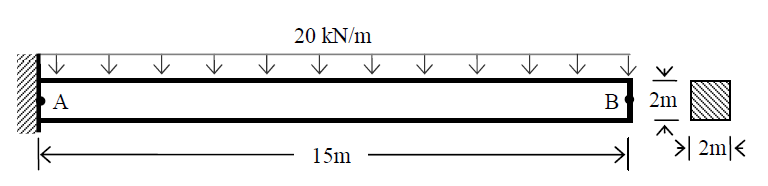
\includegraphics[width=0.65\linewidth]{figs/beam.png}
  \caption{Beam}
\end{figure}
The maximum vertical displacement of the beam in m is
\begin{multicols}{2}
\begin{enumerate}[label=(\Alph*), itemsep=0pt, topsep=2pt]
  \item 0.004
  \item 0.020
  \item 0.071
  \item 0.190
\end{enumerate}
\end{multicols}
\hfill{\brak{\text{GATE MN 2012}}}

% Q9
\item In a surface mine, sound pressure level at a location generated by operation of a dozer and a drill
respectively are $80$ dBA and $60$ dBA, when operated independently. The sound pressure generated
by the dozer compared to the drill is higher by a factor of
\begin{multicols}{2}
\begin{enumerate}[label=(\Alph*), itemsep=0pt, topsep=2pt]
  \item 10
  \item 20
  \item 100
  \item 200
\end{enumerate}
\end{multicols}
\hfill{\brak{\text{GATE MN 2012}}}

% Q10
\item As per the Indian Electricity Rules 1956, the maximum permissible length of a flexible cable used
with an electric rope shovel in m is
\begin{multicols}{2}
\begin{enumerate}[label=(\Alph*), itemsep=0pt, topsep=2pt]
  \item 100
  \item 200
  \item 300
  \item 500
\end{enumerate}
\end{multicols}
\hfill{\brak{\text{GATE MN 2012}}}
% Q11
\item The equipment that is NOT used in hard rock metal mining drivage is
\begin{multicols}{2}
\begin{enumerate}[label=(\Alph*), itemsep=0pt, topsep=2pt]
  \item road header
  \item drill jumbo
  \item jack hammer
  \item dint header
\end{enumerate}
\end{multicols}
\hfill{\brak{\text{GATE MN 2012}}}

% Q12
\item The roof bolt that follows the principle of point anchorage is
\begin{multicols}{2}
\begin{enumerate}[label=(\Alph*), itemsep=0pt, topsep=2pt]
  \item expansion shell bolt
  \item full column grouted bolt
  \item split set bolt
  \item swellex bolt
\end{enumerate}
\end{multicols}
\hfill{\brak{\text{GATE MN 2012}}}

% Q13
\item Equipment used in mining of placer deposits is
\begin{multicols}{2}
\begin{enumerate}[label=(\Alph*), itemsep=0pt, topsep=2pt]
  \item auger
  \item wagon drill
  \item rope saw
  \item riffle box
\end{enumerate}
\end{multicols}
\hfill{\brak{\text{GATE MN 2012}}}

% Q14
\item A dump truck powered by $350$ kW engine is running at a speed of $35$ km/h. Considering the
transmission efficiency of the truck as $85\%$, the rim pull of the truck in kN is
\begin{multicols}{2}
\begin{enumerate}[label=(\Alph*), itemsep=0pt, topsep=2pt]
  \item 21
  \item 31
  \item 41
  \item 51
\end{enumerate}
\end{multicols}
\hfill{\brak{\text{GATE MN 2012}}}

% Q15
\item Nystagmus is a miner’s disease associated with
\begin{multicols}{2}
\begin{enumerate}[label=(\Alph*), itemsep=0pt, topsep=2pt]
  \item lever
  \item lung
  \item eye
  \item stomach
\end{enumerate}
\end{multicols}
\hfill{\brak{\text{GATE MN 2012}}}

% Q16
\item Apart from mining of coal, the longwall mining method has been practiced for mining the deposits of
\begin{multicols}{2}
\begin{enumerate}[label=(\Alph*), itemsep=0pt, topsep=2pt]
  \item copper
  \item lead and zinc
  \item manganese
  \item pyrite and phosphate
\end{enumerate}
\end{multicols}
\hfill{\brak{\text{GATE MN 2012}}}

% Q17
\item The three segments, whose synchronous functioning is essential for GPS operations, are
\begin{multicols}{2}
\begin{enumerate}[label=(\Alph*), itemsep=0pt, topsep=2pt]
  \item space, control and user
  \item signal, control and user
  \item space, control and geo-registration
  \item signal, control and geo-registration
\end{enumerate}
\end{multicols}
\hfill{\brak{\text{GATE MN 2012}}}

% Q18
\item When a double ended ranging drum shearer cuts coal in a longwall face,
\begin{enumerate}[label=(\Alph*), itemsep=3pt, topsep=2pt]
  \item both the drums rotate in the same direction keeping the front drum up and the rear drum down
  \item both the drums rotate in the opposite direction keeping the front drum up and the rear drum down
  \item both the drums rotate in the opposite direction keeping the front drum down and the rear drum up
  \item both the drums rotate in the same direction keeping the front drum down and the rear drum up
\end{enumerate}
\hfill{\brak{\text{GATE MN 2012}}}
% Q19 (Match the following)
\item The match the following

\begin{table}[H]
\centering
\begin{tabular}{|c|c|c|}
\hline
T1 & T2 & T3 \\
\hline
\begin{minipage}{0.28\linewidth}
\begin{verbatim}
while(true){
 wait(S3);
 print("C");
 signal(S2); }
\end{verbatim}
\end{minipage}
&
\begin{minipage}{0.28\linewidth}
\begin{verbatim}
while(true){
 wait(S1);
 print("B");
 signal(S3); }
\end{verbatim}
\end{minipage}
&
\begin{minipage}{0.28\linewidth}
\begin{verbatim}
while(true){
 wait(S2);
 print("A");
 signal(S1); }
\end{verbatim}
\end{minipage}
\\
\hline
\end{tabular}
\caption*{}
\label{tab:q19}
\end{table}

\begin{multicols}{2}
\begin{enumerate}[label=(\Alph*)]
\item P-1, Q-2, R-3, S-4
\item P-3, Q-4, R-1, S-2
\item P-2, Q-1, R-4, S-3
\item P-2, Q-1, R-3, S-4
\end{enumerate}
\end{multicols}
\hfill{\brak{\text{GATE MN 2012}}}

% Q20
\item Continuous miner and shuttle car combination is NOT applicable in mining with
\begin{multicols}{2}
\begin{enumerate}[label=(\Alph*), itemsep=0pt, topsep=2pt]
  \item rib pillar extraction technique
  \item Wangawilli system
  \item room and pillar method
  \item longwall method
\end{enumerate}
\end{multicols}
\hfill{\brak{\text{GATE MN 2012}}}

% Q21
\item Contours in a topographic map
\begin{enumerate}[label=(\Alph*), itemsep=3pt, topsep=2pt]
  \item are not closed upon themselves although the earth is a continuous surface
  \item are not perpendicular to the direction of maximum slope
  \item provide an indication of presence of valley or ridge in the area
  \item are the lines joining the points of same declination at different elevations
\end{enumerate}
\hfill{\brak{\text{GATE MN 2012}}}

% Q22
\item A Dragger Gas Mask DOES NOT filter
\begin{multicols}{2}
\begin{enumerate}[label=(\Alph*), itemsep=0pt, topsep=2pt]
  \item water vapour
  \item nitrous fumes
  \item carbon monoxide
  \item carbon dioxide
\end{enumerate}
\end{multicols}
\hfill{\brak{\text{GATE MN 2012}}}

% Q23
\item A system consists of four elements A, B, C and D which are connected functionally in a parallel
configuration. The individual reliability of the elements is $0.80$, $0.82$, $0.85$ and $0.90$
respectively. The reliability of the system is
\begin{multicols}{2}
\begin{enumerate}[label=(\Alph*), itemsep=0pt, topsep=2pt]
  \item 0.498
  \item 0.602
  \item 0.750
  \item 0.999
\end{enumerate}
\end{multicols}
\hfill{\brak{\text{GATE MN 2012}}}

% Q24
\item The blasting technique used for controlled throw of overburden is known as
\begin{multicols}{2}
\begin{enumerate}[label=(\Alph*), itemsep=0pt, topsep=2pt]
  \item cast blasting
  \item coyote blasting
  \item plaster shooting
  \item pop shooting
\end{enumerate}
\end{multicols}
\hfill{\brak{\text{GATE MN 2012}}}

% Q25
\item The stoping method, where a large part of blasted ore is allowed to accumulate in the stope to
serve the purpose of providing working platform for stoping as well as to support the wall-rock,
is known as
\begin{multicols}{2}
\begin{enumerate}[label=(\Alph*), itemsep=0pt, topsep=2pt]
  \item shrinkage stoping
  \item cut and fill stoping
  \item square-set stoping
  \item sublevel stoping
\end{enumerate}
\end{multicols}
\hfill{\brak{\text{GATE MN 2012}}}\\[0.5em]
\vspace{0.3cm}
\noindent\textbf{Q.~26 to Q.~55 carry two marks each.}
\vspace{0.3cm}


% Q26
\item The injury rates of mine workers in an underground coal mine based on age group are given below:

\begin{center}
\renewcommand{\arraystretch}{1.35}
\setlength{\tabcolsep}{6pt}
\begin{tabular}{ |p{3.6cm}|p{4.4cm}|p{3.6cm}| }
  \hline
  {\centering \textbf{Age group of\\ mine workers}\par} &
  {\centering \textbf{Age-specific injury rate\\ (per 1000 persons)}\par} &
  {\centering \textbf{Age-specific population\\ in the mine}\par} \\
  \hline
  {\centering 18--32\par} & {\centering 1.8\par} & {\centering 1000\par} \\ \hline
  {\centering 33--46\par} & {\centering 2.5\par} & {\centering 500\par}  \\ \hline
  {\centering 47--60\par} & {\centering 4.5\par} & {\centering 300\par}  \\ \hline
\end{tabular}
\end{center}


The injury rate per 1000 persons employed in the mine for the total population is

\begin{multicols}{2}
\begin{enumerate}[label=(\Alph*)]
\item 0.24
\item 2.44
\item 8.80
\item 24.40
\end{enumerate}
\end{multicols}
\hfill{\brak{\text{GATE MN 2012}}}

% Q27
\item A shearer is deployed in a mine where the specific energy consumption for cutting coal is $800~\text{kJ/m}^3$. 
The specific gravity of coal is $1.2$. If the machine produces $700~\text{te/h}$, the electrical power consumption in kW of the shearer at $65\%$ motor efficiency is
\begin{multicols}{2}
\begin{enumerate}[label=(\Alph*),itemsep=0pt,topsep=2pt]
  \item 149.4
  \item 199.4
  \item 219.4
  \item 239.4
\end{enumerate}
\end{multicols}
\hfill{\brak{\text{GATE MN 2012}}}

% Q28 (figure placeholder)
\item The figure shows a weightless beam $PQ$ of length $8$ m resting on a hinge support at $P$ and on a roller support at $R$. A vertical force of $40$ N is acting at a distance of $4$ m from $P$. A uniformly distributed load of $10$ N/m is acting on a length of $2$ m of the beam from $Q$.
\begin{figure}[H]
\centering
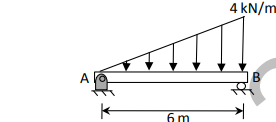
\includegraphics[width=0.6\linewidth]{figs/load.png}
\caption{Beam $PQ$ with point load and UDL.}
\end{figure}
The magnitude of reaction force at $R$ in N is
\begin{multicols}{2}
\begin{enumerate}[label=(\Alph*),itemsep=0pt,topsep=2pt]
  \item 20
  \item 30
  \item 40
  \item 50
\end{enumerate}
\end{multicols}
\hfill{\brak{\text{GATE MN 2012}}}

% Q29 (figure placeholder)
\item The figure shows the distance–time graph of a moving particle. The tangents to the curve at $A$ and $B$ make angles of $45^\circ$ and $60^\circ$ respectively with the time axis. The ratio of the speeds of the particle at $B$ and at $A$ is
\begin{figure}[H]
\centering
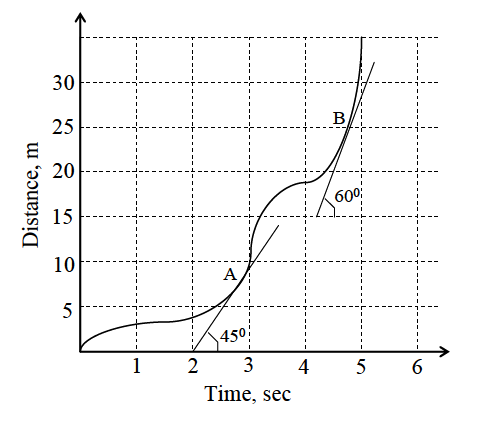
\includegraphics[width=0.6\linewidth]{figs/ratios.png}
\caption{Distance–time curve with tangents at $A$ and $B$.}
\end{figure}
\begin{multicols}{2}
\begin{enumerate}[label=(\Alph*),itemsep=0pt,topsep=2pt]
  \item 0.72
  \item 1.38
  \item 1.58
  \item 1.75
\end{enumerate}
\end{multicols}
\hfill{\brak{\text{GATE MN 2012}}}

% Q30 (figure placeholder)
\item The gear ratios of the first gear, transfer case and differential of a four wheel drive vehicle are $3.81{:}1$, $2.72{:}1$ and $4.11{:}1$ respectively. If the engine is rotating at $1000$ rpm and the wheel diameter is $1.2$ m, the speed of the vehicle in first gear in km/h is
\begin{figure}[H]
\centering
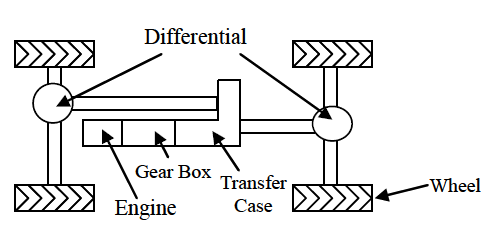
\includegraphics[width=0.55\linewidth]{figs/gearratios.png}
\caption{Engine–gearbox–transfer case–differential–wheel train.}
\end{figure}
\begin{multicols}{2}
\begin{enumerate}[label=(\Alph*),itemsep=0pt,topsep=2pt]
  \item 5.31
  \item 3.68
  \item 2.42
  \item 1.68
\end{enumerate}
\end{multicols}
\hfill{\brak{\text{GATE MN 2012}}}

% Q31
\item An iron ore mine recorded an average of 3 accidents per month. The number of accidents is distributed according to Poisson distribution. The probability that there will be exactly 2 accidents per month is
\begin{multicols}{2}
\begin{enumerate}[label=(\Alph*),itemsep=0pt,topsep=2pt]
  \item 0.22
  \item 0.30
  \item 0.43
  \item 0.67
\end{enumerate}
\end{multicols}
\hfill{\brak{\text{GATE MN 2012}}}

% Q32 (match)
\item Match the following:

\begin{center}
\renewcommand{\arraystretch}{1.25}
\begin{tabular}{ |c|c| }
\hline
\textbf{Equipment} & \textbf{Component} \\
\hline
P\; Scraper & 1\; Dribble belt \\ \hline
Q\; Dragline & 2\; Dipper stick \\ \hline
R\; Bucket wheel excavator & 3\; Fair lead \\ \hline
S\; Rope shovel & 4\; Bowl \\ \hline
\end{tabular}
\end{center}

\begin{multicols}{2}
\begin{enumerate}[label=(\Alph*),itemsep=0pt,topsep=2pt]
  \item P-2, Q-4, R-3, S-1
  \item P-4, Q-2, R-1, S-3
  \item P-4, Q-3, R-1, S-2
  \item P-2, Q-4, R-1, S-3
\end{enumerate}
\end{multicols}
\hfill{\brak{\text{GATE MN 2012}}}

% Q33
\item The torque (in N·m) of a winder motor is described by the relationship $T = 1450 - 3.2\,\omega$, where $\omega$ is the angular speed of the motor in rad/s. If the shaft is rotating at a speed of 1450 rpm, the power of the motor in kW is
\begin{multicols}{2}
\begin{enumerate}[label=(\Alph*),itemsep=0pt,topsep=2pt]
  \item 112.4
  \item 146.4
  \item 184.4
  \item 212.4
\end{enumerate}
\end{multicols}
\hfill{\brak{\text{GATE MN 2012}}}

% Q34
\item An investment of Rs.\ 10{,}000, compounded annually, is estimated to return Rs.\ 20{,}000 after 6 years from the date of investment. The expected rate of return on this investment in percentage is
\begin{multicols}{2}
\begin{enumerate}[label=(\Alph*),itemsep=0pt,topsep=2pt]
  \item 8.75
  \item 10.50
  \item 12.25
  \item 16.6
\end{enumerate}
\end{multicols}
\hfill{\brak{\text{GATE MN 2012}}}

% Q35
\item A spherical droplet of water, with density $1000~\text{kg/m}^3$ and diameter of $1~\mu\text{m}$, is falling in air. The viscosity of air is $1.85\times10^{-5}~\text{kg/(m·s)}$. Neglecting air density and assuming that the settling of droplet in air follows Stokes’ Law, the settling velocity in m/s is
\begin{multicols}{2}
\begin{enumerate}[label=(\Alph*),itemsep=0pt,topsep=2pt]
  \item $0.98\times10^{-5}$
  \item $2.95\times10^{-5}$
  \item $8.04\times10^{-5}$
  \item $53.03\times10^{-5}$
\end{enumerate}
\end{multicols}
\hfill{\brak{\text{GATE MN 2012}}}


% Q36
\item A mining company has three mines (M1, M2 and M3) that supply coal to three
power plants (P1, P2 and P3). The three mines produce 900, 1000 and 1200 te of
coal per day respectively. The power plant requirements from these three mines
are 1200, 1000 and 900 te per day respectively. The unit cost of transporting
coal from the three mines to the three power plants in Rs. is given below

\begin{circuitikz}
\draw (0,0) to[V=$V_I$] (0,2) to[R=$R$] (2,2) to[zzD] (2,0) to[R=1k$\Omega$] (2,-2) node[ground] {};
\draw (2,2) to[short,-o] (3,2) node[above] {5V};
\end{circuitikz}
 % <- table file

Based on the initial basic feasible solution, using Vogel’s approximation
method, the total transportation cost in Rs. is

\begin{multicols}{2}
\begin{enumerate}[label=(\Alph*),itemsep=0pt,topsep=2pt]
\item 31200
\item 31400
\item 32800
\item 40000
\end{enumerate}
\end{multicols}
\hfill{\brak{\text{GATE MN 2012}}}

% Q37
\item The angle between the tangents to the curve $\vec{R}=t^{2}\,\hat{i}+t\,\hat{j}$ at the points $t=\pm 1$ is
\begin{multicols}{2}
\begin{enumerate}[label=(\Alph*),itemsep=0pt,topsep=2pt]
  \item $\dfrac{\pi}{2}$
  \item $\dfrac{\pi}{3}$
  \item $\dfrac{\pi}{4}$
  \item $\dfrac{\pi}{6}$
\end{enumerate}
\end{multicols}
\hfill{\brak{\text{GATE MN 2012}}}

% Q38


\item The chip sampling data, spaced irregularly for a gold vein deposit, are shown in figure.
The sample points have equal influence on both the sides.

% Keep this if you want the table separately.
\begin{tabular}{|l|l|}
\hline
\textbf{Ecological observations} & \textbf{Processes} \\
\hline
P) Bright spotted pigmentation in & I) Kin selection \\
guppy males in low predation habitats & \\
\hline
Q) Vampire bats share blood meals & II) Sexual selection \\
\hline
R) Cooperative breeding in African & III) Reciprocal altruism \\
weaver birds & \\
\hline
\end{tabular} \\

% Replace the drawn TikZ with a single image file
\begin{center}
  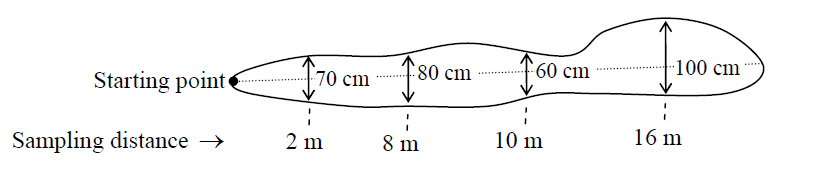
\includegraphics[width=0.9\linewidth]{figs/q38} % figs/q38.png or figs/q38.pdf
\end{center}

The mean assay value in g/te is

\begin{multicols}{2}
\begin{enumerate}[label=(\Alph*),itemsep=0pt,topsep=2pt]
  \item 6.52
  \item 5.50
  \item 5.19
  \item 4.50
\end{enumerate}
\end{multicols}
\hfill{\brak{\text{GATE MN 2012}}}



% Q39
\item A series of triaxial tests of sandstone samples reveal the cohesion and the angle of internal friction as $21.65$ MPa and $30^\circ$ respectively. Based on Mohr–Coulomb failure criterion, the tensile strength in MPa is
\begin{multicols}{2}
\begin{enumerate}[label=(\Alph*),itemsep=0pt,topsep=2pt]
  \item 12.50
  \item 18.75
  \item 21.65
  \item 25.00
\end{enumerate}
\end{multicols}
\hfill{\brak{\text{GATE MN 2012}}}

% Q40
\item The adjusted values of departure and latitude for a traverse line $AB$ obtained in a field survey are $225.520$ m and $388.835$ m respectively. The length in m and azimuth of line $AB$ are
\begin{multicols}{2}
\begin{enumerate}[label=(\Alph*),itemsep=0pt,topsep=2pt]
  \item 449.50, $30.11^\circ$
  \item 614.36, $30.11^\circ$
  \item 614.36, $45.11^\circ$
  \item 449.50, $45.11^\circ$
\end{enumerate}
\end{multicols}
\hfill{\brak{\text{GATE MN 2012}}}

% Q41
\item The figure shows the values of seven perpendicular offsets and the respective locations along the line $XY$ as observed while carrying out a traverse survey. The area of the plot $XABCDEFGY$ in m$^2$ is
\begin{figure}[H]
\centering
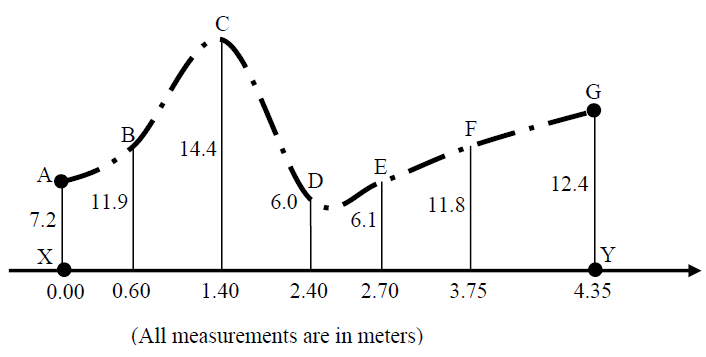
\includegraphics[width=0.7\linewidth]{figs/offsets.png}
\caption{Perpendicular offsets along line $XY$.}
\end{figure}
\begin{multicols}{2}
\begin{enumerate}[label=(\Alph*),itemsep=0pt,topsep=2pt]
  \item 26.10
  \item 43.38
  \item 44.92
  \item 62.50
\end{enumerate}
\end{multicols}
\hfill{\brak{\text{GATE MN 2012}}}

% Q42
\item In a longwall panel, the main gate road is 1000 m long, 4.5 m wide and 2 m high. The gate road is to be used for airflow at the rate of $17~\text{m}^3/\text{s}$. Considering a coefficient of resistance of airways of $0.01$, the pressure in Pa required to maintain the airflow in the gate road is
\begin{multicols}{2}
\begin{enumerate}[label=(\Alph*),itemsep=0pt,topsep=2pt]
  \item 51.83
  \item 463.84
  \item 875.98
  \item 7885.32
\end{enumerate}
\end{multicols}
\hfill{\brak{\text{GATE MN 2012}}}

% Q43
\item The cofactor matrix of 
$\displaystyle P=\myvec{3 & 1 & 2\\[2pt] 2 & 3 & 1\\[2pt] 1 & 2 & 3}$ is
\begin{multicols}{2}
\begin{enumerate}[label=(\Alph*),itemsep=2pt,topsep=2pt]
  \item $\myvec{-21 & -5 & -2\\ -2 & -21 & -5\\ -5 & -2 & -21}$
  \item $\myvec{-21 & -2 & -5\\ -2 & \;\;\,7 & \;\,15\\ -5 & \;\,21 & \;\,2}$
  \item $\myvec{-5 & -2 & -21\\ -15 & -7 & -2\\ \;\,2 & \;\,21 & \;\,5}$
  \item $\myvec{\;\,15 & \;\,7 & \;\,2\\ -5 & -2 & -21\\ \;\,2 & \;\,21 & \;\,5}$
\end{enumerate}
\end{multicols}
\hfill{\brak{\text{GATE MN 2012}}}

% Q44
\setcounter{enumi}{43}
\item Match the following:

\begin{center}
\renewcommand{\arraystretch}{1.25}
\setlength{\tabcolsep}{4pt} % tighter side padding
\small
\begin{tabular}{ |p{0.58\linewidth}|p{0.36\linewidth}| }
  \hline
  \textbf{Mining system} & \textbf{Face supports} \\ \hline
  {\raggedright P\; Mechanized longwall in flat seam\par} &
  {\raggedright 1\; Cable bolting\par} \\ \hline
  {\raggedright Q\; Blasting gallery method\par} &
  {\raggedright 2\; Shield support\par} \\ \hline
  {\raggedright R\; Mechanized longwall in steep seam\par} &
  {\raggedright 3\; Alpine breaker line support\par} \\ \hline
  {\raggedright S\; Wangawilli method for 3 m thick coal seam\par} &
  {\raggedright 4\; Troika shield support\par} \\ \hline
\end{tabular}
\normalsize
\end{center}
 % <- table file

\begin{multicols}{2}
\begin{enumerate}[label=(\Alph*),itemsep=0pt,topsep=2pt]
  \item P-2, Q-1, R-4, S-3
  \item P-4, Q-1, R-3, S-2
  \item P-4, Q-2, R-3, S-1
  \item P-2, Q-3, R-4, S-1
\end{enumerate}
\end{multicols}
\hfill{\brak{\text{GATE MN 2012}}}
\newpage
% Q45
\item An opencast mine bench has a potential failure plane $AC$ as indicated in the figure. Bolts are installed to stabilize the failure plane providing a resultant bolting force of $300$ kN. The area of sliding block $ABC$ is $37.45~\text{m}^2$. The unit weight, cohesion and angle of internal friction of rock are $25~\text{kN/m}^3$, $20$ kPa and $40^\circ$ respectively. The factor of safety of slope when bolts are installed perpendicular to the failure plane is
\begin{figure}[H]
\centering
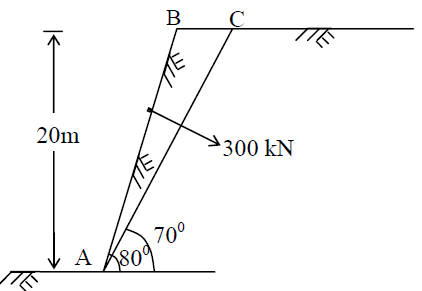
\includegraphics[width=0.55\linewidth]{figs/opencast.png}
\caption{Potential failure plane $AC$ and bolting.}
\end{figure}
\begin{multicols}{2}
\begin{enumerate}[label=(\Alph*),itemsep=0pt,topsep=2pt]
  \item 0.79
  \item 1.08
  \item 1.78
  \item 3.46
\end{enumerate}
\end{multicols}
\hfill{\brak{\text{GATE MN 2012}}}
\newpage
% Q46
\item Figure shows a two pulley system for hoisting a load of $10$ kN. The coefficient of friction between each pulley and the rope is $0.2$. The vertical and horizontal distances between the centers of the pulleys are $25$ m and $16$ m respectively. The tensions $T_1$ and $T_2$ respectively in kN are
\begin{figure}[H]
\centering
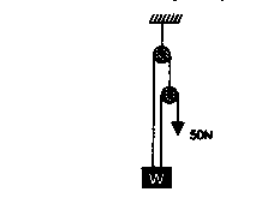
\includegraphics[width=0.6\linewidth]{figs/pulley.png}
\caption{Two-pulley hoist with friction.}
\end{figure}
\begin{multicols}{2}
\begin{enumerate}[label=(\Alph*),itemsep=0pt,topsep=2pt]
  \item 6.00, 5.38
  \item 12.37, 11.06
  \item 18.74, 16.73
  \item 25.11, 22.41
\end{enumerate}
\end{multicols}
\hfill{\brak{\text{GATE MN 2012}}}

% Q47
\item A circular tunnel of $1.85$ m radius is driven in rock in a hydrostatic stress field of $20$ MPa. The tunnel lining is provided before occurrence of any rock deformation. The shear modulus of rock is $2$ GPa and the modulus of elasticity of lining material is $3$ GPa. Assuming both rock and lining behave elastically, the radial pressure on the rock–lining interface in MPa is
\begin{multicols}{2}
\begin{enumerate}[label=(\Alph*),itemsep=0pt,topsep=2pt]
  \item 8.19
  \item 9.91
  \item 11.62
  \item 13.33
\end{enumerate}
\end{multicols}
\hfill{\brak{\text{GATE MN 2012}}}



% ---------- Q48 & Q49 : Common Data ----------
\noindent\textbf{Common Data for Q.48 and Q.49:}
A $2.5$ m thick coal seam lying at an average depth of $100$ m has been developed by bord and pillar method.
The width of the square pillars is $30$ m (centre to centre) and the gallery width is $4$ m.
The average density of the overlying strata is $26~\text{kN/m}^3$ and the pillar strength is $4500~\text{kN/m}^2$.

% Q48
\item The extraction ratio during the development of the panel is
\begin{multicols}{2}
\begin{enumerate}[label=(\Alph*), itemsep=0pt, topsep=2pt]
  \item 0.129
  \item 0.148
  \item 0.218
  \item 0.249
\end{enumerate}
\end{multicols}
\hfill{\brak{\text{GATE MN 2012}}}

% Q49
\item The safety factor of the pillar (w.r.t. overburden load) is
\begin{multicols}{2}
\begin{enumerate}[label=(\Alph*), itemsep=0pt, topsep=2pt]
  \item 1.1
  \item 1.3
  \item 1.5
  \item 1.7
\end{enumerate}
\end{multicols}
\hfill{\brak{\text{GATE MN 2012}}}

% ---------- Q50 & Q51 : Common Data ----------
\noindent\textbf{Common Data for Q.50 and Q.51:}\\[0.5em] The following data are provided for a surface mine to be excavated by a shovel:\\[0.5em]
Production target: $10000$ te/shift;\\[0.5em] \; Available hours per shift: $6$ h;\\[0.5em] \; Shovel loading cycles per hour: $106$;\\[0.5em]\\
Bank density: $2400~\text{kg/m}^3$;\\[0.5em] \; Swing factor at $120^\circ$: $0.91$;\\[0.5em] \; Bucket fill factor: $0.64$;\\[0.5em]\\
Utilization of available time: $83\%$;\\[0.5em] \; Working days/year: $300$;\\[0.5em] \; Shifts/day: $3$.\\[0.5em]

% Q50
\item The annual production target in Mte is
\begin{multicols}{2}
\begin{enumerate}[label=(\Alph*), itemsep=0pt, topsep=2pt]
  \item 5.76
  \item 7.00
  \item 8.19
  \item 9.00
\end{enumerate}
\end{multicols}
\hfill{\brak{\text{GATE MN 2012}}}

% Q51
\item The required bucket size of the shovel in m$^3$ is
\begin{multicols}{2}
\begin{enumerate}[label=(\Alph*), itemsep=0pt, topsep=2pt]
  \item 5.55
  \item 9.33
  \item 11.22
  \item 13.55
\end{enumerate}
\end{multicols}
\hfill{\brak{\text{GATE MN 2012}}}

% ---------- Q52 & Q53 : Linked Answer (PERT) ----------
\noindent\textbf{Linked Answer Questions Q.52 and Q.53:}\\
A mining project is composed of five activities whose three time estimates (months) are:


\begin{center}
\begin{tabular}[12pt]{ |c| c| c| c| }
\hline
\textbf{Activity} & \textbf{Optimistic} & \textbf{Most likely} & \textbf{Permissible}\\
\hline
1--2 & 1 & 1 & 7\\
\hline
1--3 & 2 & 5 & 8\\
\hline
2--4 & 1 & 1 & 7\\
\hline
3--4 & 2 & 5 & 14\\
\hline
4--5 & 3 & 6 & 15\\
\hline
\end{tabular}
\end{center} % <- table file
% Q52
\item The expected duration of the project (months) is
\begin{multicols}{2}
\begin{enumerate}[label=(\Alph*), itemsep=0pt, topsep=2pt]
  \item 5
  \item 16
  \item 18
  \item 29
\end{enumerate}
\end{multicols}
\hfill{\brak{\text{GATE MN 2012}}}

% Q53
\item The standard deviation of the project length (months) is
\begin{multicols}{2}
\begin{enumerate}[label=(\Alph*), itemsep=0pt, topsep=2pt]
  \item 2
  \item 3
  \item 6
  \item 9
\end{enumerate}
\end{multicols}
\hfill{\brak{\text{GATE MN 2012}}}

% ---------- Q54 & Q55 : Linked Answer (Ventilation) ----------
\noindent\textbf{Statement for Linked Answer Questions Q.54 and Q.55:}\\
Between upcast and downcast shafts, two parallel airways have resistances $100$ and $120~\text{N\,s}^{-2}\text{m}^{-8}$.
Resistances of upcast shaft, downcast shaft and fan drifts are $10$, $20$ and $5~\text{N\,s}^{-2}\text{m}^{-8}$ respectively.
The fan develops an air power (pressure) of $15$ MN/m$^2$.

% Q54
\item The rate of airflow through the mine in m$^3$/s is
\begin{multicols}{2}
\begin{enumerate}[label=(\Alph*), itemsep=0pt, topsep=2pt]
  \item 4.16
  \item 18.26
  \item 240.35
  \item 333.33
\end{enumerate}
\end{multicols}
\hfill{\brak{\text{GATE MN 2012}}}

% Q55
\item The airflow through the split airway of resistance $100~\text{N\,s}^{-2}\text{m}^{-8}$ in m$^3$/s is
\begin{multicols}{2}
\begin{enumerate}[label=(\Alph*), itemsep=0pt, topsep=2pt]
  \item 0.42
  \item 0.79
  \item 2.19
  \item 7.90
\end{enumerate}
\end{multicols}
\hfill{\brak{\text{GATE MN 2012}}}

% ---- GA header ----
\noindent\textbf{General Aptitude (GA) Questions}\\
\noindent Q.\ 56--Q.\ 60 carry one mark each.

% Q56
\item Choose the most appropriate alternative from the options given below to complete the following sentence: \\
I \_\_\_\_\_ to have bought a diamond ring.
\begin{multicols}{2}
\begin{enumerate}[label=(\Alph*), itemsep=0pt, topsep=2pt]
  \item have a liking
  \item should have liked
  \item would like
  \item may like
\end{enumerate}
\end{multicols}
\hfill{\brak{\text{GATE MN 2012}}}

% Q57
\item Choose the most appropriate alternative from the options given below to complete the following sentence: \\
Food prices \_\_\_\_\_ again this month.
\begin{multicols}{2}
\begin{enumerate}[label=(\Alph*), itemsep=0pt, topsep=2pt]
  \item have raised
  \item have been raising
  \item have been rising
  \item have arose
\end{enumerate}
\end{multicols}
\hfill{\brak{\text{GATE MN 2012}}}

% Q58
\item Choose the most appropriate alternative from the options given below to complete the following sentence: \\
The administrators went on to implement yet another unreasonable measure, arguing that the measures were already \_\_\_\_\_ and one more would hardly make a difference.
\begin{multicols}{2}
\begin{enumerate}[label=(\Alph*), itemsep=0pt, topsep=2pt]
  \item reflective
  \item utopian
  \item luxuriant
  \item unpopular
\end{enumerate}
\end{multicols}
\hfill{\brak{\text{GATE MN 2012}}}

% Q59
\item Choose the most appropriate alternative from the options given below to complete the following sentence: \\
To those of us who had always thought him timid, his \_\_\_\_\_ came as a surprise.
\begin{multicols}{2}
\begin{enumerate}[label=(\Alph*), itemsep=0pt, topsep=2pt]
  \item intrepidity
  \item inevitability
  \item inability
  \item inertness
\end{enumerate}
\end{multicols}
\hfill{\brak{\text{GATE MN 2012}}}

% Q60
\item The arithmetic mean of five different natural numbers is 12. The largest possible value among the numbers is
\begin{multicols}{2}
\begin{enumerate}[label=(\Alph*), itemsep=0pt, topsep=2pt]
  \item 12
  \item 40
  \item 50
  \item 60
\end{enumerate}
\end{multicols}
\hfill{\brak{\text{GATE MN 2012}}}\\[0.5em]
\noindent Q.\ 61--Q.\ 65 carry two marks each.

% Q61
\item Two policemen, A and B, fire once each at the same time at an escaping convict. The probability that A hits the convict is three times the probability that B hits the convict. If the probability of the convict not getting injured is 0.5, the probability that B hits the convict is
\begin{multicols}{2}
\begin{enumerate}[label=(\Alph*), itemsep=0pt, topsep=2pt]
  \item 0.14
  \item 0.22
  \item 0.33
  \item 0.40
\end{enumerate}
\end{multicols}
\hfill{\brak{\text{GATE MN 2012}}}

% Q62
\item The total runs scored by four cricketers P, Q, R, and S in years 2009 and 2010 are given in the following table. The player with the lowest percentage increase in total runs is

\begin{center}
\begin{tabular}[12pt]{ |c| c| c| }
\hline
\textbf{Player} & \textbf{2009} & \textbf{2010}\\
\hline
P & 802 & 1008\\
\hline
Q & 765 & 912\\
\hline
R & 429 & 619\\
\hline
S & 501 & 701\\
\hline
\end{tabular}
\end{center}
 % <-- separate table file

\begin{multicols}{2}
\begin{enumerate}[label=(\Alph*), itemsep=0pt, topsep=2pt]
  \item P
  \item Q
  \item R
  \item S
\end{enumerate}
\end{multicols}
\hfill{\brak{\text{GATE MN 2012}}}


% Q63
\item If a prime number on division by 4 gives a remainder of 1, then that number can be expressed as
\begin{enumerate}[label=(\Alph*), itemsep=0pt, topsep=2pt]
  \item sum of squares of two natural numbers
  \item sum of cubes of two natural numbers
  \item sum of square roots of two natural numbers
  \item sum of cube roots of two natural numbers
\end{enumerate}
\hfill{\brak{\text{GATE MN 2012}}}

% Q64
\item Two points $(4, p)$ and $(0, q)$ lie on a straight line having a slope of $3/4$. The value of $(p - q)$ is
\begin{multicols}{2}
\begin{enumerate}[label=(\Alph*), itemsep=0pt, topsep=2pt]
  \item $-3$
  \item $0$
  \item $3$
  \item $4$
\end{enumerate}
\end{multicols}
\hfill{\brak{\text{GATE MN 2012}}}

% Q65
\item In the early nineteenth century, theories of social evolution were inspired less by Biology than by the conviction of social scientists that there was a growing improvement in social institutions. Progress was taken for granted and social scientists attempted to discover its laws and phases. \\
Which one of the following inferences may be drawn with the greatest accuracy from the above passage? Social scientists
\begin{enumerate}[label=(\Alph*), itemsep=0pt, topsep=2pt]
  \item did not question that progress was a fact.
  \item did not approve of Biology.
  \item framed the laws of progress.
  \item emphasized Biology over Social Sciences.
\end{enumerate}
\hfill{\brak{\text{GATE MN 2012}}}

\end{enumerate}

\begin{center}
    \textbf{END OF THE QUESTION PAPER}
\end{center}
\end{enumerate}
\end{document}